% Options for packages loaded elsewhere
\PassOptionsToPackage{unicode}{hyperref}
\PassOptionsToPackage{hyphens}{url}
%
\documentclass[
  14pt,
  a5paper,
]{extarticle}
\usepackage{amsmath,amssymb}
\usepackage{iftex}
\ifPDFTeX
  \usepackage[T1]{fontenc}
  \usepackage[utf8]{inputenc}
  \usepackage{textcomp} % provide euro and other symbols
\else % if luatex or xetex
  \usepackage{unicode-math} % this also loads fontspec
  \defaultfontfeatures{Scale=MatchLowercase}
  \defaultfontfeatures[\rmfamily]{Ligatures=TeX,Scale=1}
\fi
\usepackage{lmodern}
\ifPDFTeX\else
  % xetex/luatex font selection
  \setmainfont[]{Noto Sans CJK JP}
  \setsansfont[]{Noto Sans CJK JP}
  \setmonofont[]{Noto Sans Mono CJK JP}
\fi
% Use upquote if available, for straight quotes in verbatim environments
\IfFileExists{upquote.sty}{\usepackage{upquote}}{}
\IfFileExists{microtype.sty}{% use microtype if available
  \usepackage[]{microtype}
  \UseMicrotypeSet[protrusion]{basicmath} % disable protrusion for tt fonts
}{}
\makeatletter
\@ifundefined{KOMAClassName}{% if non-KOMA class
  \IfFileExists{parskip.sty}{%
    \usepackage{parskip}
  }{% else
    \setlength{\parindent}{0pt}
    \setlength{\parskip}{6pt plus 2pt minus 1pt}}
}{% if KOMA class
  \KOMAoptions{parskip=half}}
\makeatother
\usepackage{xcolor}
\usepackage[margin=12mm]{geometry}
\usepackage{color}
\usepackage{fancyvrb}
\newcommand{\VerbBar}{|}
\newcommand{\VERB}{\Verb[commandchars=\\\{\}]}
\DefineVerbatimEnvironment{Highlighting}{Verbatim}{commandchars=\\\{\}}
% Add ',fontsize=\small' for more characters per line
\newenvironment{Shaded}{}{}
\newcommand{\AlertTok}[1]{\textcolor[rgb]{1.00,0.00,0.00}{\textbf{#1}}}
\newcommand{\AnnotationTok}[1]{\textcolor[rgb]{0.38,0.63,0.69}{\textbf{\textit{#1}}}}
\newcommand{\AttributeTok}[1]{\textcolor[rgb]{0.49,0.56,0.16}{#1}}
\newcommand{\BaseNTok}[1]{\textcolor[rgb]{0.25,0.63,0.44}{#1}}
\newcommand{\BuiltInTok}[1]{\textcolor[rgb]{0.00,0.50,0.00}{#1}}
\newcommand{\CharTok}[1]{\textcolor[rgb]{0.25,0.44,0.63}{#1}}
\newcommand{\CommentTok}[1]{\textcolor[rgb]{0.38,0.63,0.69}{\textit{#1}}}
\newcommand{\CommentVarTok}[1]{\textcolor[rgb]{0.38,0.63,0.69}{\textbf{\textit{#1}}}}
\newcommand{\ConstantTok}[1]{\textcolor[rgb]{0.53,0.00,0.00}{#1}}
\newcommand{\ControlFlowTok}[1]{\textcolor[rgb]{0.00,0.44,0.13}{\textbf{#1}}}
\newcommand{\DataTypeTok}[1]{\textcolor[rgb]{0.56,0.13,0.00}{#1}}
\newcommand{\DecValTok}[1]{\textcolor[rgb]{0.25,0.63,0.44}{#1}}
\newcommand{\DocumentationTok}[1]{\textcolor[rgb]{0.73,0.13,0.13}{\textit{#1}}}
\newcommand{\ErrorTok}[1]{\textcolor[rgb]{1.00,0.00,0.00}{\textbf{#1}}}
\newcommand{\ExtensionTok}[1]{#1}
\newcommand{\FloatTok}[1]{\textcolor[rgb]{0.25,0.63,0.44}{#1}}
\newcommand{\FunctionTok}[1]{\textcolor[rgb]{0.02,0.16,0.49}{#1}}
\newcommand{\ImportTok}[1]{\textcolor[rgb]{0.00,0.50,0.00}{\textbf{#1}}}
\newcommand{\InformationTok}[1]{\textcolor[rgb]{0.38,0.63,0.69}{\textbf{\textit{#1}}}}
\newcommand{\KeywordTok}[1]{\textcolor[rgb]{0.00,0.44,0.13}{\textbf{#1}}}
\newcommand{\NormalTok}[1]{#1}
\newcommand{\OperatorTok}[1]{\textcolor[rgb]{0.40,0.40,0.40}{#1}}
\newcommand{\OtherTok}[1]{\textcolor[rgb]{0.00,0.44,0.13}{#1}}
\newcommand{\PreprocessorTok}[1]{\textcolor[rgb]{0.74,0.48,0.00}{#1}}
\newcommand{\RegionMarkerTok}[1]{#1}
\newcommand{\SpecialCharTok}[1]{\textcolor[rgb]{0.25,0.44,0.63}{#1}}
\newcommand{\SpecialStringTok}[1]{\textcolor[rgb]{0.73,0.40,0.53}{#1}}
\newcommand{\StringTok}[1]{\textcolor[rgb]{0.25,0.44,0.63}{#1}}
\newcommand{\VariableTok}[1]{\textcolor[rgb]{0.10,0.09,0.49}{#1}}
\newcommand{\VerbatimStringTok}[1]{\textcolor[rgb]{0.25,0.44,0.63}{#1}}
\newcommand{\WarningTok}[1]{\textcolor[rgb]{0.38,0.63,0.69}{\textbf{\textit{#1}}}}
\usepackage{longtable,booktabs,array}
\usepackage{calc} % for calculating minipage widths
% Correct order of tables after \paragraph or \subparagraph
\usepackage{etoolbox}
\makeatletter
\patchcmd\longtable{\par}{\if@noskipsec\mbox{}\fi\par}{}{}
\makeatother
% Allow footnotes in longtable head/foot
\IfFileExists{footnotehyper.sty}{\usepackage{footnotehyper}}{\usepackage{footnote}}
\makesavenoteenv{longtable}
\usepackage{graphicx}
\makeatletter
\def\maxwidth{\ifdim\Gin@nat@width>\linewidth\linewidth\else\Gin@nat@width\fi}
\def\maxheight{\ifdim\Gin@nat@height>\textheight\textheight\else\Gin@nat@height\fi}
\makeatother
% Scale images if necessary, so that they will not overflow the page
% margins by default, and it is still possible to overwrite the defaults
% using explicit options in \includegraphics[width, height, ...]{}
\setkeys{Gin}{width=\maxwidth,height=\maxheight,keepaspectratio}
% Set default figure placement to htbp
\makeatletter
\def\fps@figure{htbp}
\makeatother
\setlength{\emergencystretch}{3em} % prevent overfull lines
\providecommand{\tightlist}{%
  \setlength{\itemsep}{0pt}\setlength{\parskip}{0pt}}
\setcounter{secnumdepth}{-\maxdimen} % remove section numbering
\usepackage{setspace,needspace,etoolbox}
\setstretch{1.12}
\XeTeXlinebreaklocale "ja"
\XeTeXlinebreakskip=0pt plus 1pt
\setlength{\parindent}{0pt}
\setlength{\parskip}{0.24em}
\setlength{\footskip}{18pt}
\renewcommand{\arraystretch}{1.08}
\pretocmd{\section}{\Needspace{5\baselineskip}}{}{}
\usepackage{fvextra}
\newcommand{\commutecodefont}{\fontsize{10}{12}\selectfont}
\DefineVerbatimEnvironment{Highlighting}{Verbatim}{breaklines,fontsize=\commutecodefont,commandchars=\\\{\}}
\renewcommand{\CommentTok}[1]{\textcolor[rgb]{0.25,0.25,0.25}{#1}}
\makeatletter
\renewcommand{\maketitle}{\begin{center}\vspace*{-5mm}{\LARGE\bfseries\@title\par}\vspace{3mm}{\normalsize\@date\par}\end{center}}
\makeatother
\ifLuaTeX
  \usepackage{selnolig}  % disable illegal ligatures
\fi
\usepackage{bookmark}
\IfFileExists{xurl.sty}{\usepackage{xurl}}{} % add URL line breaks if available
\urlstyle{same}
\hypersetup{
  pdftitle={自分の実験を 説明するための読み物},
  hidelinks,
  pdfcreator={LaTeX via pandoc}}

\title{自分の実験を 説明するための読み物}
\usepackage{etoolbox}
\makeatletter
\providecommand{\subtitle}[1]{% add subtitle to \maketitle
  \apptocmd{\@title}{\par {\large #1 \par}}{}{}
}
\makeatother
\subtitle{実験の回数・結果・式・コードを順番に理解する}
\author{}
\date{2026年11月27日}

\begin{document}
\maketitle

\textbf{電車で読むための解説版}

提出レポートの内容を，自分の言葉で説明できるようにするための資料である．

最初に「何を何回して，どうなったか」を読み，次に式とコードをつなげて理解する．

\begin{itemize}
\tightlist
\item
  1〜5：実験内容・回数・結果
\item
  6〜8：入力とニューラルネットワーク
\item
  9〜13：学習・損失・枝刈り
\item
  14〜17：CSRと保存容量
\item
  18〜21：MSE・計時・説明の練習
\item
  22：回路図と入出力ピン
\end{itemize}

コードは使用済みソースの抜粋を中心に掲載した．説明用の数値・疑似コードはその旨を記した．画像と説明はPDFに入っているため，保存後はオフラインで読める．

\newpage

\section{1　何を調べた実験か}\label{ux4f55ux3092ux8abfux3079ux305fux5b9fux9a13ux304b}

\textbf{色補正モデルを小さく・速くしても，色の正確さを保てるかを調べた．}

Arduino UNO R4
WiFiで，紙から読み取ったRGBをニューラルネットワークで補正した．比較した方式は2つである．

\textbf{Dense}は，全ての重みを保存して計算する通常方式．\textbf{枝刈り＋CSR}は，小さい重みを0にし，残った値と位置を保存して計算する方式である．

隠れ層の大きさHを40・60・80・100としたので，4種類×2方式＝\textbf{8条件}になる．

説明するときは，次の内容を軸にする．

「同じ読取入力を8条件へ与え，色の誤差・モデル容量・計算時間を比較しました．容量と時間は減りましたが，圧縮後の誤差は増え，精度維持の目標は達成しませんでした．」

\newpage

\section{2　何を何回したか}\label{ux4f55ux3092ux4f55ux56deux3057ux305fux304b}

\textbf{学習}：過去の実測135組を使用した．3×3分111組と6×4分24組で，同じ色の繰り返しも含む．各Hの保存済みモデルから\textbf{40,000回ずつ追加更新}した．

\textbf{閾値選択}：別の8×8チャートを\textbf{2回}読んだ128入力を使用した．

\textbf{精度比較}：9色を最後まで読む操作を\textbf{10回}行った．新しい読取入力は90組で，MSEは8条件×10回＝80個である．

\textbf{速度測定}：各条件で準備運転10回後，\textbf{100推論×5組}を計時した．計時対象は1条件500推論，全8条件で4,000推論である．

\textbf{単独メモリ比較}：8条件を1条件ずつ，それぞれ1回コンパイルしてIDE表示を記録した．

学習の更新回数，紙の読取回数，保存入力の再生回数は分けて数える．

\newpage

\section{3　紙を読むときの手順}\label{ux7d19ux3092ux8aadux3080ux3068ux304dux306eux624bux9806}

各回で黒・白を登録し，入力の基準を合わせた．その後，赤・緑・青・黄・水色・紫・黒・灰・白の順に読み取った．


\includegraphics[width=38mm,height=\textheight]{../color_images/reference.png}

\begin{center}
正解RGBの9色（result.ppm）
\end{center}

\textbf{1回の読取値を，全8条件で共有した．}
方式ごとに紙を読み直したものではない．

9色終了時に，8枚のPPMと8個のMSEを保存した．これを10回行い，PPM80枚・MSE80個を得た．

各RGB成分では10サンプルを平均したが，実験の反復単位は「9色を読み終える1回」である．

新規10回ではモデルと閾値を固定し，その読取値を学習へ追加していない．紙の色自体は学習時と同じである．

\newpage

\section{4　精度はどうなったか}\label{ux7cbeux5ea6ux306fux3069ux3046ux306aux3063ux305fux304b}

次の値は，全10回を含めた平均MSEである．\textbf{小さいほど正解に近い．}

\begin{longtable}[]{@{}lrr@{}}
\toprule\noalign{}
H & Dense & 枝刈り＋CSR \\
\midrule\noalign{}
\endhead
\bottomrule\noalign{}
\endlastfoot
40 & 319.56 & 452.04 \\
60 & 238.33 & 493.51 \\
80 & 231.68 & 465.72 \\
100 & 260.42 & 651.92 \\
\end{longtable}

DenseのH60・80・100は平均300以下だった．CSRは全Hで平均300を超えた．同じ回で比べても，全H・全10回でCSRのMSEが大きかった．

H60
Denseは，10回目の画像ではMSEが\textbf{2.33}だったが，第2回は\textbf{2339.37}だった．全10回平均は\textbf{238.33}となる．

良かった1回の画像のMSEと，10回平均は別の値である．第2回も含めて集計し，除外した回はない．

本書のMSE表示は小数第2位までとし，第3位以降を切り捨てている．

\newpage

\section{5　容量・速度・RAMの結果}\label{ux5bb9ux91cfux901fux5ea6ramux306eux7d50ux679c}

H60で，Denseから枝刈り＋CSRへ変えると次のようになった．

\textbf{モデルの数値配列}

16,332 → 6,449 byte\\
約60.51\%削減

\textbf{1推論の計算時間}

945.648 → 671.674 µs\\
約28.97\%短縮

\textbf{単独プログラム全体のFlash}

69,492 → 59,612 byte\\
約14.22\%削減

\textbf{静的RAM}

両方式とも6,764 byteで，同じだった．

モデル配列だけの容量と，Arduinoの基本処理を含むFlash全体は分けて比較する．実行時スタックの最大使用量は未測定である．

\newpage

\section{6　入力をそろえる正規化}\label{ux5165ux529bux3092ux305dux308dux3048ux308bux6b63ux898fux5316}

黒の基準を0，白の基準を1とするため，次の式を使う．レポートの式(1)に対応する．

\[x=\frac{\text{読取値}-\text{黒の値}}{\text{白の値}-\text{黒の値}}\]

実際の1回目の赤成分では，

\[\frac{137.5-9.8}{186.4-9.8}\approx0.7231\]

となった．ログのNN入力R＝0.7231はこの結果である．

\texttt{normalizeInput()}の中心部分を抜粋する．

\begin{Shaded}
\begin{Highlighting}[]
\DataTypeTok{float}\NormalTok{ range }\OperatorTok{=}
\NormalTok{  whiteValue }\OperatorTok{{-}}\NormalTok{ blackValue}\OperatorTok{;}
\DataTypeTok{float}\NormalTok{ result }\OperatorTok{=}
  \OperatorTok{(}\NormalTok{value }\OperatorTok{{-}}\NormalTok{ blackValue}\OperatorTok{)}
  \OperatorTok{/}\NormalTok{ range}\OperatorTok{;}
\end{Highlighting}
\end{Shaded}

その後，0未満を0，1を超えた値を1に収める．これがクリップである．白−黒が0以下のときは，関数は0を返す．

この段階では入力の尺度をそろえ，次に学習済みモデルで色を補正する．

\newpage

\section{7　重み・バイアス・ReLU}\label{ux91cdux307fux30d0ux30a4ux30a2ux30b9relu}

\textbf{重みw}は，入力を何倍して使うかを決める係数．\textbf{バイアスb}は，合計へ加える調整値である．

\[z=w_Rx_R+w_Gx_G+w_Bx_B+b\]

説明用に入力(0.7,0.2,0.1)，重み(0.5,−0.2,0.3)，バイアス0.01とすると，

\[z=0.35-0.04+0.03+0.01=0.35\]

となる．負の重みは，入力の影響を差し引く方向に働く．

隠れ層では，この合計をReLUへ通す．

\[\operatorname{ReLU}(z)=\max(0,z)\]

0.35なら0.35，−0.2なら0になる．出力層は線形で，最後のRGB変換時にクリップする．

学習では，正解に近い色が出るように重みとバイアスを更新する．

\newpage

\section{8　Denseの構造とコード}\label{denseux306eux69cbux9020ux3068ux30b3ux30fcux30c9}

構造は「3入力→H個→H個→3出力」．H60なら，各隠れ層に60個の計算単位がある．

接続1本に重みが1個あるため，H60の重み数は，

\[3\times60+60\times60+60\times3=3,960\]

バイアスは60＋60＋3＝123個である．

最初の隠れ層の計算コードを抜粋する．

\begin{Shaded}
\begin{Highlighting}[]
\DataTypeTok{float}\NormalTok{ value}\OperatorTok{=}\NormalTok{m}\OperatorTok{.}\NormalTok{b1}\OperatorTok{[}\NormalTok{r}\OperatorTok{];}
\ControlFlowTok{for}\OperatorTok{(}\DataTypeTok{int}\NormalTok{ c}\OperatorTok{=}\DecValTok{0}\OperatorTok{;}\NormalTok{c}\OperatorTok{\textless{}}\DecValTok{3}\OperatorTok{;}\NormalTok{c}\OperatorTok{++)}\NormalTok{ value}\OperatorTok{+=}\NormalTok{m}\OperatorTok{.}\NormalTok{w1}\OperatorTok{[}\NormalTok{r}\OperatorTok{*}\DecValTok{3}\OperatorTok{+}\NormalTok{c}\OperatorTok{]*}\NormalTok{input}\OperatorTok{[}\NormalTok{c}\OperatorTok{];}
\NormalTok{layer1}\OperatorTok{[}\NormalTok{r}\OperatorTok{]=}\NormalTok{value}\OperatorTok{\textgreater{}}\FloatTok{0.0}\BuiltInTok{f}\OperatorTok{?}\NormalTok{value}\OperatorTok{:}\FloatTok{0.0}\BuiltInTok{f}\OperatorTok{;}
\end{Highlighting}
\end{Shaded}

\texttt{r}は計算単位の番号，\texttt{c}はRGBの番号．バイアスから始め，入力と重みの積を足す．\texttt{+=}は「今の値へ加える」の意味である．

最後の\texttt{条件\ ?\ A\ :\ B}は，条件が成立すればA，成立しなければBを選ぶ．ここではReLUを実装している．

\newpage

\section{9　学習の式は何の採点か}\label{ux5b66ux7fd2ux306eux5f0fux306fux4f55ux306eux63a1ux70b9ux304b}

学習では，予測色の間違いを減らし，重みも大きくしすぎないようにする．レポートの式(5)は，この合計点を表す．

\[\mathcal L=A+10^{-6}B\]

\textbf{A：色の誤差の重要度付き平均}

各行のRGB誤差を平均した点数を \(E_i\)，その行の重要度を \(a_i\)
とすると，

\[A=\frac{1}{\sum_{i=1}^{135}a_i}\sum_{i=1}^{135}a_iE_i\]

\textbf{B：全3層の重みの絶対値の合計}

\[B=\sum_{\ell=1}^{3}\sum_{j,k}|(W_\ell)_{jk}|\]

\(\mathcal L\)が小さくなる方向へ重みを更新する．AとBの内容を，次の2ページで確認する．

これは学習時の損失であり，結果表の整数RGBのMSEとは計算方法が異なる．

\newpage

\section{10　Smooth
L1の式とコード}\label{smooth-l1ux306eux5f0fux3068ux30b3ux30fcux30c9}

予測−正解をeとする．誤差の点数には，次のSmooth
L1を使った．\(\beta=0.05\)である．

\[\rho_\beta(e)=\begin{cases}e^2/(2\beta)&(|e|<\beta),\\|e|-\beta/2&(|e|\geq\beta)\end{cases}\]

2つの式を足すのではなく，条件に合う片方を使う．説明用に，

\begin{itemize}
\tightlist
\item
  e＝0.02なら，\(0.02^2/0.1=0.004\)
\item
  e＝0.1なら，\(0.1-0.025=0.075\)
\end{itemize}

となる．大きな残差の影響を抑えるため，小さい誤差では二乗，大きい誤差では直線的に増やす．

学習コードの対応部分は次である．

\begin{Shaded}
\begin{Highlighting}[]
\NormalTok{loss\_rows }\OperatorTok{=}\NormalTok{ F.smooth\_l1\_loss(}
\NormalTok{    prediction, ty,}
\NormalTok{    beta}\OperatorTok{=}\FloatTok{.05}\NormalTok{, reduction}\OperatorTok{=}\StringTok{\textquotesingle{}none\textquotesingle{}}
\NormalTok{).mean(}\DecValTok{1}\NormalTok{)}
\end{Highlighting}
\end{Shaded}

\texttt{prediction}は予測，\texttt{ty}は正解RGBを255で割った値．\texttt{.mean(1)}はRGBの3成分を平均し，1行分の誤差点数を作る．

\newpage

\section{11　重要度とL1の意味}\label{ux91cdux8981ux5ea6ux3068l1ux306eux610fux5473}

\(a_i\)は学習データの行ごとの重要度で，ネットワークの重みWとは別の値である．

説明用に，誤差点数が2と4，重要度が1と3なら，平均は，

\[\frac{1\times2+3\times4}{1+3}=3.5\]

となる．最初の分子が1なのは「重要度の合計で割る」ためで，各行の \(a_i\)
はその誤差へ掛ける．

L1では全重みの絶対値を合計する．重みが0.1，−0.2，0なら，合計は0.3，罰則は，

\[10^{-6}\times0.3=0.0000003\]

である．外側のシグマは層，内側は各層の全重みを足す．バイアスは罰則から除いた．

L1は小さな重みを作る方向に作用する．重みを実際に0へ変えるのは，後の枝刈りである．

\newpage

\section{12　学習コードの読み方}\label{ux5b66ux7fd2ux30b3ux30fcux30c9ux306eux8aadux307fux65b9}

使用した\texttt{train.py}から，中心部分を抜粋する．長い式は折り返して表示している．

\begin{Shaded}
\begin{Highlighting}[]
\NormalTok{optimizer.zero\_grad()}\OperatorTok{;}\NormalTok{prediction}\OperatorTok{=}\NormalTok{model(ax)}
\NormalTok{loss\_rows}\OperatorTok{=}\NormalTok{F.smooth\_l1\_loss(prediction,ty,beta}\OperatorTok{=}\FloatTok{.05}\NormalTok{,reduction}\OperatorTok{=}\StringTok{\textquotesingle{}none\textquotesingle{}}\NormalTok{).mean(}\DecValTok{1}\NormalTok{)}
\NormalTok{loss}\OperatorTok{=}\NormalTok{(loss\_rows}\OperatorTok{*}\NormalTok{weights).}\BuiltInTok{sum}\NormalTok{()}\OperatorTok{/}\NormalTok{weights.}\BuiltInTok{sum}\NormalTok{()}\OperatorTok{+}\FloatTok{1e{-}6}\OperatorTok{*}\BuiltInTok{sum}\NormalTok{(p.}\BuiltInTok{abs}\NormalTok{().}\BuiltInTok{sum}\NormalTok{() }\ControlFlowTok{for}\NormalTok{ name,p }\KeywordTok{in}\NormalTok{ model.named\_parameters() }\ControlFlowTok{if} \StringTok{\textquotesingle{}weight\textquotesingle{}} \KeywordTok{in}\NormalTok{ name)}
\ControlFlowTok{assert}\NormalTok{ torch.isfinite(loss)}\OperatorTok{;}\NormalTok{loss.backward()}\OperatorTok{;}\NormalTok{optimizer.step()}\OperatorTok{;}\NormalTok{schedule.step()}
\end{Highlighting}
\end{Shaded}

\texttt{zero\_grad()}で前回の勾配を消し，\texttt{model(ax)}で今回の予測を出す．\texttt{ax}は学習時の入力で，データ拡張を含む．

\texttt{loss\_rows}は各行のRGB誤差．次の行の前半は重要度付き平均，後半はL1の罰則である．\texttt{weights}は行の重要度で，\texttt{p}はモデル内の学習パラメータを表す．

\texttt{\textquotesingle{}weight\textquotesingle{}\ in\ name}により，L1へ重みだけを含める．\texttt{backward()}で勾配を求め，\texttt{step()}でAdamによる更新を行う．\texttt{isfinite}は異常値の検査，\texttt{schedule.step()}は学習率の更新を行う．

勾配は，重みなどを動かしたときに損失がどちらへ変わるかを示す値である．その情報から，損失を減らす方向へ更新する．

この更新を各Hで40,000回行った．入力例を学習で繰り返す回数であり，紙を40,000回測ったものではない．

\newpage

\section{13　枝刈りと閾値選択}\label{ux679dux5208ux308aux3068ux95beux5024ux9078ux629e}

枝刈りは，絶対値が閾値 \(\tau\) より小さい重みを0にする処理である．

\[|w|<\tau\quad\Rightarrow\quad w=0\]

H60の閾値は約0.05434179だった．例えば0.03，−0.02は0となり，0.2は残る．バイアスは保持する．

1個の重みの判定を，説明用の疑似コードで書くと次になる．

\begin{Shaded}
\begin{Highlighting}[]
\ControlFlowTok{if} \BuiltInTok{abs}\NormalTok{(w) }\OperatorTok{\textless{}}\NormalTok{ tau:}
\NormalTok{    w }\OperatorTok{=} \DecValTok{0}
\end{Highlighting}
\end{Shaded}

候補は学習済み重みの値から作った．別の8×8チャート2回分の128入力で，MSE増加5\%以下かつ小容量となるものを残した．学習内9入力でMSE300以下も満たす候補から，最小容量を選んだ．

新規10回の開始前に固定し，その結果による選び直しは行っていない．\(\tau\)とSmooth
L1の \(\beta\) は用途が異なる．

\newpage

\section{14　CSRのvaluesとcol}\label{csrux306evaluesux3068col}

以下は仕組みを説明する2行3列の例である．番号は0から数える．

\begin{Shaded}
\begin{Highlighting}[]
\NormalTok{        列0   列1  列2}
\NormalTok{行0      0    0.5   0}
\NormalTok{行1    {-}0.2    0   0.1}
\end{Highlighting}
\end{Shaded}

上の行から，0以外の値とその列番号を追加する．

\begin{Shaded}
\begin{Highlighting}[]
\NormalTok{values = [0.5, {-}0.2, 0.1]}
\NormalTok{col    = [1,    0,   2  ]}
\end{Highlighting}
\end{Shaded}

保存位置kをそろえて読む．

\begin{itemize}
\tightlist
\item
  k＝0：値0.5は，元の列1にあった
\item
  k＝1：値−0.2は，元の列0にあった
\item
  k＝2：値0.1は，元の列2にあった
\end{itemize}

\textbf{valuesの何番目かと，元の列番号は別の番号である．}

値と列だけでは行の区切りが分からないので，次のページのrowも保存する．

\newpage

\section{15　CSRのrowと計算範囲}\label{csrux306erowux3068ux8a08ux7b97ux7bc4ux56f2}

前ページの例では，行の開始位置を次のように保存する．

\begin{Shaded}
\begin{Highlighting}[]
\NormalTok{values = [0.5, {-}0.2, 0.1]}
\NormalTok{row    = [0,    1,   3  ]}
\end{Highlighting}
\end{Shaded}

行rで使うのは，\textbf{row{[}r{]}からrow{[}r＋1{]}の手前まで}である．

\begin{itemize}
\tightlist
\item
  行0：0番から1番の手前 → k＝0
\item
  行1：1番から3番の手前 → k＝1，2
\end{itemize}

最後の3は終端で，values{[}3{]}を読む指定ではない．rowの要素数は「行数＋1」になる．

説明用に入力(1,2,3)，バイアス0とすると，colを使って，

\[\text{行0}=0.5\times2=1\]

\[\text{行1}=-0.2\times1+0.1\times3=0.1\]

となる．CSRでは，値・列・行の区切りを組み合わせて，0を省いた積和計算を行う．

\newpage

\section{16　CSR推論コードの読み方}\label{csrux63a8ux8ad6ux30b3ux30fcux30c9ux306eux8aadux307fux65b9}

使用した\texttt{sparseLayer()}の本体を抜粋し，改行を整えて示す．

\begin{Shaded}
\begin{Highlighting}[]
\ControlFlowTok{for} \OperatorTok{(}\DataTypeTok{int}\NormalTok{ r}\OperatorTok{=}\DecValTok{0}\OperatorTok{;}\NormalTok{ r}\OperatorTok{\textless{}}\NormalTok{layer}\OperatorTok{.}\NormalTok{rows}\OperatorTok{;}\NormalTok{ r}\OperatorTok{++)} \OperatorTok{\{}
  \DataTypeTok{float}\NormalTok{ value}\OperatorTok{=}\NormalTok{layer}\OperatorTok{.}\NormalTok{bias}\OperatorTok{[}\NormalTok{r}\OperatorTok{];}
  \ControlFlowTok{for} \OperatorTok{(}\DataTypeTok{uint16\_t}\NormalTok{ k}\OperatorTok{=}\NormalTok{layer}\OperatorTok{.}\NormalTok{row}\OperatorTok{[}\NormalTok{r}\OperatorTok{];}
\NormalTok{       k}\OperatorTok{\textless{}}\NormalTok{layer}\OperatorTok{.}\NormalTok{row}\OperatorTok{[}\NormalTok{r}\OperatorTok{+}\DecValTok{1}\OperatorTok{];}\NormalTok{ k}\OperatorTok{++)}
\NormalTok{    value }\OperatorTok{+=}\NormalTok{ layer}\OperatorTok{.}\NormalTok{values}\OperatorTok{[}\NormalTok{k}\OperatorTok{]}
           \OperatorTok{*}\NormalTok{ input}\OperatorTok{[}\NormalTok{layer}\OperatorTok{.}\NormalTok{col}\OperatorTok{[}\NormalTok{k}\OperatorTok{]];}
\NormalTok{  output}\OperatorTok{[}\NormalTok{r}\OperatorTok{]=(}\NormalTok{relu }\OperatorTok{\&\&}\NormalTok{ value}\OperatorTok{\textless{}}\DecValTok{0}\OperatorTok{)}
          \OperatorTok{?} \DecValTok{0} \OperatorTok{:}\NormalTok{ value}\OperatorTok{;}
\OperatorTok{\}}
\end{Highlighting}
\end{Shaded}

外側の\texttt{for}は出力先の各行を計算する．\texttt{value}をバイアスで初期化し，内側の\texttt{for}でその行に残った重みだけを使う．

\texttt{layer.values{[}k{]}}を，\texttt{layer.col{[}k{]}}が示す入力へ掛けて足す．最後に，\texttt{relu}が有効で値が負なら0とする．

\texttt{input{[}...{]}}や\texttt{row{[}...{]}}の角括弧は，配列の指定位置を読む記号である．\texttt{k++}はkを1増やす．\texttt{float}は小数，\texttt{int}は整数を扱う型である．

\newpage

\section{17　保存容量の式を読む}\label{ux4fddux5b58ux5bb9ux91cfux306eux5f0fux3092ux8aadux3080}

FP32は数値1個に4
byte使う．H60では重み3,960個，バイアス123個なので，Denseは，

\[(3,960+123)\times4=16,332\ \text{byte}\]

CSRではK＝1,141個を残した．

\begin{longtable}[]{@{}lr@{}}
\toprule\noalign{}
保存するもの & H60の容量 \\
\midrule\noalign{}
\endhead
\bottomrule\noalign{}
\endlastfoot
重みvalues：4K & 4,564 byte \\
列番号col：K & 1,141 byte \\
行位置row & 252 byte \\
バイアス & 492 byte \\
\end{longtable}

rowは61＋61＋4＝126個×2 byteである．一般式と合計は次になる．

\[B_{\mathrm{CSR}}=4K+K+2(2H+6)+4(2H+3)\]

\[B_{\mathrm{CSR}}=6,449\ \text{byte}\]

位置情報にも容量が必要であり，重みが十分減らないとCSRの容量は小さくならない．

\newpage

\section{18　MSEの式とコード}\label{mseux306eux5f0fux3068ux30b3ux30fcux30c9}

モデルの出力を0〜1へ収め，255倍して四捨五入し，整数RGBに変換する．正解との差を二乗して平均する．

\[\mathrm{MSE}=\frac1{27}\sum_{i=1}^{9}\sum_{c\in\{R,G,B\}}(y_{i,c}-t_{i,c})^2\]

9色×3成分なので27で割る．説明用に，1色だけが正解(255,0,0)，予測(245,10,5)で，他の8色が一致した場合，

\[\mathrm{MSE}=\frac{100+100+25}{27}=8.33\ldots\]

となる．保存入力版のMSE計算から抜粋する．

\begin{Shaded}
\begin{Highlighting}[]
\DataTypeTok{int}\NormalTok{ e}\OperatorTok{=}\KeywordTok{static\_cast}\OperatorTok{\textless{}}\DataTypeTok{int}\OperatorTok{\textgreater{}(}
\NormalTok{  pixels}\OperatorTok{[}\NormalTok{model}\OperatorTok{][}\NormalTok{point}\OperatorTok{][}\NormalTok{c}\OperatorTok{])}
  \OperatorTok{{-}}\NormalTok{trained\_models}\OperatorTok{::}\NormalTok{REFERENCE\_RGB}\OperatorTok{[}\NormalTok{point}\OperatorTok{][}\NormalTok{c}\OperatorTok{];}
\NormalTok{mse}\OperatorTok{[}\NormalTok{model}\OperatorTok{]+=}\KeywordTok{static\_cast}\OperatorTok{\textless{}}\DataTypeTok{double}\OperatorTok{\textgreater{}(}\NormalTok{e}\OperatorTok{)*}\NormalTok{e}\OperatorTok{/}\FloatTok{27.0}\OperatorTok{;}
\end{Highlighting}
\end{Shaded}

\texttt{e}は整数RGBの差．\texttt{static\_cast}は型変換で，二乗を小数型\texttt{double}で計算している．各成分の二乗を27で割って加算する．RGBへの四捨五入と，MSE表示の小数第3位以降の切り捨ては，別の処理である．

\newpage

\section{19　平均・SD・差・増加率}\label{ux5e73ux5747sdux5deeux5897ux52a0ux7387}

各回のMSEを \(m_r\) とすると，10回平均は，

\[\overline m=\frac{m_1+\cdots+m_{10}}{10}\]

標本SDは各回が平均からどれだけ離れたかを表す．標本SDの定義に従い10−1＝9で割る．

\[s_m=\sqrt{\frac{\sum_{r=1}^{10}(m_r-\overline m)^2}{9}}\]

同じ回の差は
\(d_r=m_{r,\mathrm{CSR}}-m_{r,\mathrm{Dense}}\)．正なら圧縮後に誤差が増えたことを示す．

MSE増加率は平均同士の比から求める．

\[100\left(\frac{\overline m_{\mathrm{CSR}}}{\overline m_{\mathrm{Dense}}}-1\right)\]

説明用に100→130なら30\%増加．今回の精度維持条件は5\%以下だった．一方，容量・時間は減った割合を見るため，\(100(1-\text{圧縮後}/\text{圧縮前})\)で削減率を求める．

\newpage

\section{20　速度測定コードを読む}\label{ux901fux5ea6ux6e2cux5b9aux30b3ux30fcux30c9ux3092ux8aadux3080}

\texttt{timeModel()}の計時部分を抜粋し，改行を整えて示す．

\begin{Shaded}
\begin{Highlighting}[]
\DataTypeTok{float}\NormalTok{ output}\OperatorTok{[}\DecValTok{3}\OperatorTok{];}\NormalTok{ checksum}\OperatorTok{=}\DecValTok{0}\OperatorTok{;}
\DataTypeTok{uint32\_t}\NormalTok{ begin}\OperatorTok{=}\KeywordTok{static\_cast}\OperatorTok{\textless{}}\DataTypeTok{uint32\_t}\OperatorTok{\textgreater{}(}\NormalTok{micros}\OperatorTok{());}
\ControlFlowTok{for} \OperatorTok{(}\DataTypeTok{int}\NormalTok{ call}\OperatorTok{=}\DecValTok{0}\OperatorTok{;}\NormalTok{ call}\OperatorTok{\textless{}}\DecValTok{100}\OperatorTok{;}\NormalTok{ call}\OperatorTok{++)} \OperatorTok{\{}
  \DataTypeTok{int}\NormalTok{ input}\OperatorTok{=(}\NormalTok{group}\OperatorTok{*}\DecValTok{100}\OperatorTok{+}\NormalTok{call}\OperatorTok{)}
    \OperatorTok{\%}\NormalTok{ comparison\_models}\OperatorTok{::}\NormalTok{BENCHMARK\_INPUT\_COUNT}\OperatorTok{;}
\NormalTok{  comparison\_models}\OperatorTok{::}\NormalTok{predict}\OperatorTok{(}
\NormalTok{    model}\OperatorTok{,}
\NormalTok{    comparison\_models}\OperatorTok{::}\NormalTok{BENCHMARK\_INPUTS}\OperatorTok{[}\NormalTok{input}\OperatorTok{],}
\NormalTok{    output}\OperatorTok{);}
\NormalTok{  checksum}\OperatorTok{+=}\NormalTok{output}\OperatorTok{[}\DecValTok{0}\OperatorTok{]+}\NormalTok{output}\OperatorTok{[}\DecValTok{1}\OperatorTok{]+}\NormalTok{output}\OperatorTok{[}\DecValTok{2}\OperatorTok{];}
\OperatorTok{\}}
\ControlFlowTok{return} \KeywordTok{static\_cast}\OperatorTok{\textless{}}\DataTypeTok{uint32\_t}\OperatorTok{\textgreater{}(}\NormalTok{micros}\OperatorTok{()){-}}\NormalTok{begin}\OperatorTok{;}
\end{Highlighting}
\end{Shaded}

\texttt{micros()}はµs単位の時刻を返し，終了−開始で経過時間を求める．\texttt{uint32\_t}は32bitの符号なし整数である．\texttt{\%}は余りで，保存した9入力を巡回する番号を作る．\texttt{checksum}へ出力を合計して計算結果を使う．

返るのは100推論分の時間で，呼出元で100で割る．5組の平均を結果とした．計時区間は入力選択と出力合計を含み，センサ読取・シリアル表示・MSE計算を除く．

保存入力の再生で計算時間を比較し，紙の新規10回では色の誤差を比較した．

\newpage

\section{21　質問されたときの答え方}\label{ux8ceaux554fux3055ux308cux305fux3068ux304dux306eux7b54ux3048ux65b9}

\textbf{どんな実験？}

「色補正モデルを，小さく・速くしながら精度を保てるか調べました．隠れ層40・60・80・100で，Denseと枝刈り＋CSRを比較しました．」

\textbf{何を何回？}

「9色の紙を10回読み，同じ入力を全8条件へ与えてMSE80個を得ました．速度は各条件100推論×5組，メモリは8条件の単独コンパイルで比較しました．」

\textbf{成功したことは？}

モデル配列容量と計算時間，単独Flashは減少した．静的RAMは変わらなかった．

\textbf{達成できなかったことは？}

CSRの10回平均MSE300以下と，Denseに対するMSE増加5\%以下を満たさなかった．

今回の範囲は学習チャートの新規読取での比較である．未知色の独立最終評価，H50，搭載限界と最大スタック使用量は未実施である．

\newpage

\section{22　回路図}\label{ux56deux8defux56f3}

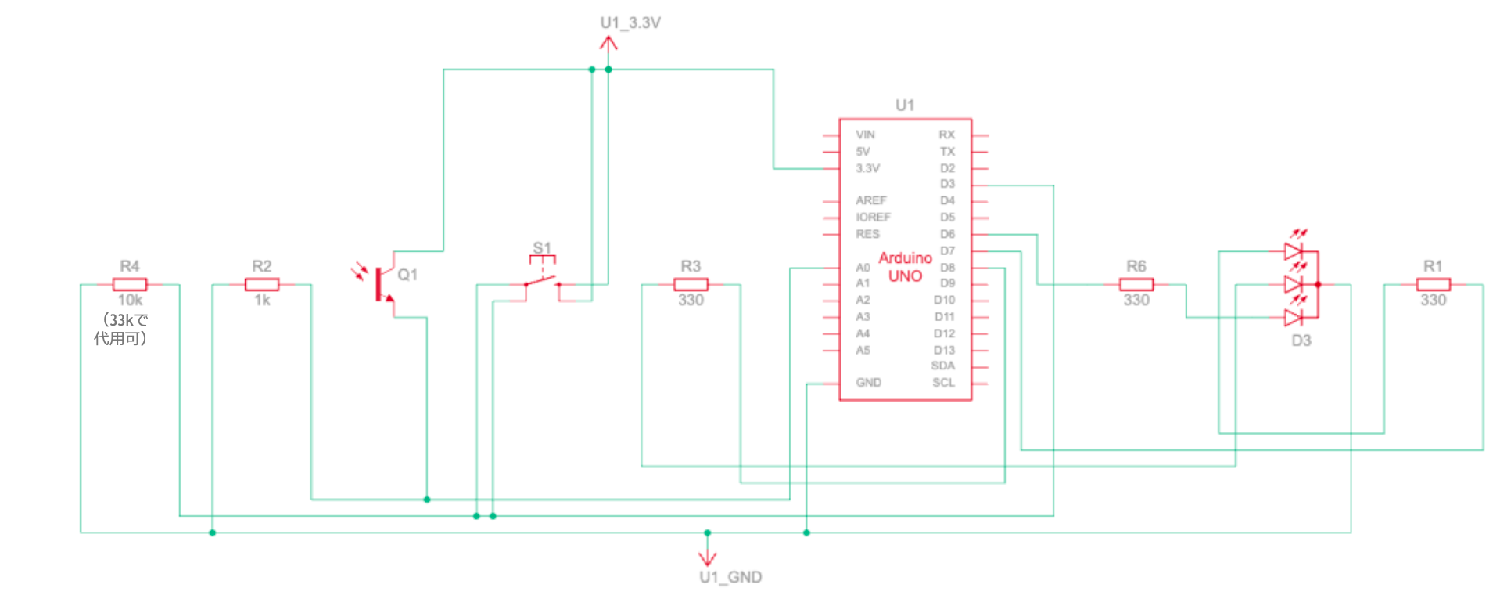
\includegraphics[width=1\textwidth,height=\textheight]{../figures/circuit.pdf}

\begin{center}
回路図
\end{center}

受け取った回路図の画像を，変更せずに掲載した．PDF内の図は拡大して読める．

\textbf{使用コードの入出力}：A0で受光電圧を読み，LEDを赤D8・緑D6・青D7から順に点灯させる．

実機の操作用入力はD2（黒白校正）とD3（色読取）で，各入力に10
kΩのプルダウン抵抗を接続した．

実測10回はシリアル操作で行い，外付けボタンは使用していない．

\end{document}
